\documentclass[11pt, letterpaper]{article}

\usepackage[authoryear]{natbib}
\usepackage{amsmath}
\usepackage{anysize}
\usepackage[colorlinks=true,urlcolor=blue,citecolor=blue]{hyperref}
\usepackage{graphicx}

\marginsize{.5in}{.5in}{.5in}{.5in}

\begin{document}
% Force pdflatex to use correct paper size.
\special{papersize=8.5in,11in}
\setlength{\pdfpageheight}{\paperheight}
\setlength{\pdfpagewidth}{\paperwidth}

\begin{center}
  {\LARGE \textbf{The Heat Equation in Fortran 90}\\}
  {\large D. T. Welling, \today}
\end{center}

Let's apply Fortran to a real-world problem: solving the 1D heat equation.
This example is taken from \citet{Mathews2004}, Example 10.3.  Let's start
with the heat equation itself:

\begin{equation}
  \label{eq:heat}
  \frac{\partial U}{\partial t} = c^2 \frac{\partial^2 U}{\partial x^2}
\end{equation}
...where $U$ is temperature as a function of location, $x$, and time, $t$; $c^2$
is thermal diffusivity.
We want to solve this equation from $0 \leq x \leq 1$ over the time
interval $t=0$ to $t=0.2$.  We want to use the following boundary
and initial conditions:

\begin{gather}
  \label{eq:boundx}
  U(0,t) = U(1, t) = 0 \\
  \label{eq:boundt}
  U(x,0) = 4x - 4x^2
\end{gather}

Of course, we cannot solve this analytically using Fortran.  We need to use
a numerical approximation.  Let's start with first- and second- order
approximations for time and spatial derivatives over a time step of
$\Delta t$ and a spatial step of $\Delta x$:

\begin{align}
  \label{eq:dif1}
  \frac{\partial U(x,t)}{\partial t}&=\frac{U(x, t+\Delta t)-U(x,t)}{\Delta t}
  +\mathcal{O}(\Delta t)\\
  \label{eq:dif2}
  \frac{\partial^2 U(x,t)}{\partial x^2}&=
  \frac{U(x-\Delta x,t)-2U(x,t)+U(x+\Delta x,t)}{\Delta x^2}
  +\mathcal{O}(\Delta x^2)
\end{align}

Equation \ref{eq:dif1} is the \emph{forward difference} formula for
obtaining a first-order accurate estimation of the first derivative.
It requires information of the function of which we are taking the
derivative, $U(x,t)$, both at the point that we want the derivative and
some point \emph{forward} of that ($U(x,t+\Delta t)$).
Equation \ref{eq:dif2} is the \emph{central-difference} formula for
a second-order accurate estimate of
the second derivative of $U(x,t)$.  It requires information both before and
after the point of interest (our derivative is given at the center of
three points: $U(x-\Delta x, t)$, $U(x,t)$, and $U(x+\Delta x, t)$).  The
derivation of these formula can be found in Chapter 6 of \citet{Mathews2004}.

Let's introduce some shorthand to make this more readable:
\begin{gather}
  h \equiv \Delta x \\
  k \equiv \Delta t
\end{gather}

If we divide up our computational domain (Equations \ref{eq:dif1}-\ref{eq:dif2}) using our
time and spatial steps, we can create a grid in space in time over which will
will obtain our solution: $x_1, x_2, \cdots x_n$ and $t_1, t_2 \cdots t_m$.
With these definitions, the solution at any point $x=x_i$ and $t=t_j$
can be expressed as $U_{i, j}$.

Inserting Equations \ref{eq:dif1}-\ref{eq:dif2} into Equation \ref{eq:heat} allows us to
gather all $U_{x,t+1}$ terms (terms that are $+\Delta t$ in the future) on
one side and all $U_{x,t}$ on the other.  This is left as an exercise for the
reader.

\begin{gather}
  \label{eq:scheme}
  U_{i, j+1} = \left(1-2r\right)U_{i,j}+r\left(U_{i-1,j}+U_{i+1,j}\right)\\
  r \equiv c^2 \frac{\Delta t}{\Delta x^2}
\end{gather}

Note that this is an \emph{explicit} method: we only need information at
$j$ to move to $j+1$.  Our scheme becomes unstable if the following criteria is
not met:

\begin{equation}
  \label{eq:cfl}
  \Delta t \leq \frac{\Delta x^2}{2c^2}
\end{equation}

Figure \ref{fig:sten} shows the \emph{stencil diagram} for this simple method,
known as the \emph{forward difference method}.  The blue dots in this
diagram show us the points where we are solving the heat equation as a function
of distance in our single dimension (``X'' on the vertical axis) and as
a function of time (horizontal axis).  The space between the dots shows us
our time and spatial steps.  At the outset, we know our initial condition,
$U_{i, j=0}$, and our boundary conditions, $U_{i=0, j}$ and $U_{i=n, j}$.
The red lines show us the flow of information
required to integrate in time: if we know the solution at a point in space-time,
$U_{i,j}$, and we want to advance the solution $\Delta t$ foward in time
($U_{i,j+1}$), we need to know not only $U_{i,j}$, but also the value at both
spatial neighbors: $U_{i\pm1,j}$.  The stencil diagram gives us clues about
how to organize our Fortran90 program.

\begin{figure}[ht!]
  \centering
  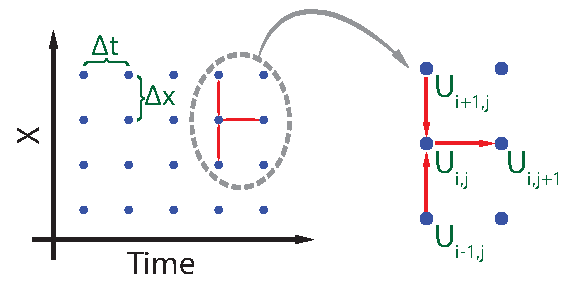
\includegraphics{./heateq_fwddiff.pdf}
  \caption{The stencil diagram for the foward difference method.  Blue dots
    represent the solution grid as a function of time (horizontal axis)
    and ``X'', the
    spatial distance along our domain (vertical axis).  The red lines show
    the flow of information required to advance from $U_{i,j}$ to $U_{i,j+1}$}  
  \label{fig:sten}
\end{figure}


The task of our program is to take these statements and put them into array form.
This tells us how our code will work.  Let's start with a 2-D array (space and
time).  We'll call it {\tt domain}.  Let {\tt domain(1, j)} and
{\tt domain(n, j)} be the upper and lower boundaries as defined by
Equation \ref{eq:boundx}.  Remember than $n$ is the number of spatial points in
our domain.  We also have our initial conditions from \ref{eq:boundt}, which
dictates the values at {\tt domain(:,1)}.  Therefore, \ref{eq:scheme} can
be re-written in Fortran 90 like so:

\begin{verbatim}
domain(2:nx-1, j+1) = (1-2r) * domain(2:nX-1, j) + 
                           r *(domain(1:nX-2, j) + domain(3:nx,j))
\end{verbatim}

We shall loop through time to accomplish this.  We now have a good idea how to
tackle the problem, but let's flesh it out further.

\begin{enumerate}
\item Initialize our problem:
  \begin{itemize}
  \item Choose end time in seconds.
  \item Set time and grid step.
  \item Determine size of domain (number of points).
  \item Create {\tt xGrid} array, fill with locations of grid points.
  \item Create {\tt domain} array that is large enough to hold the
    entire domain in both space and time. Initialize values to zero.
  \item Set initial conditions (i.e., {\tt domain(:,1)}) equal to our
    given functional value.
  \end{itemize}
\item Check stability criterion, stop if bad choice of $\Delta t$ and $\Delta x$.
\item Loop through time, solving across all $x$ at each timestep.
\item Write results to file, including timestep, grid step, and size of domain.
  \begin{itemize}
  \item Open file and assign file unit.
  \item Write a \emph{useful} header that includes size of domain, number of
    points, etc.
  \item Write grid points to file.
  \item For each time, write the time and solution over all locations.
  \end{itemize}

\item Clean up: close files, deallocate any allocated arrays.
  
\end{enumerate}

The implementation can be found in {\tt heateq\_simple.f90}.  Compile and run
this program using the folling commands at the bash command line:

\begin{verbatim}
gfortran -o heat.exe heateq_simple.f90 
./heat.exe 
\end{verbatim}

For comparison, the correct solution can be found in {\tt results\_correct.txt}.
Our current implementation works, but is the simplest implementation and is
very inflexible.  We will revisit this program and make it more modular.

\bibliographystyle{plainnat}
\bibliography{refs}

\end{document}
